\chapter{Ecological Foundations of the Niche}

\begin{objetivos}
By the end of this chapter, readers should be able to:
\begin{itemize}
  \item understand the ecological basis of species distribution modeling (SDM) and ecological niche modeling (ENM);
  \item distinguish the Grinnellian, Eltonian, and Hutchinsonian concepts of the niche;
  \item distinguish the fundamental niche, realized niche, observed distribution, and potential distribution;
  \item recognize how abiotic, biotic, and historical factors shape species distributions;
  \item critically interpret environmental-suitability maps and climate-change projections; and
  \item explain why niche conservatism is a central assumption in spatial and temporal projections.
\end{itemize}
\end{objetivos}

\section{Introduction}

Species distribution modeling (SDM), also referred to as habitat suitability
modeling (HSM) or ecological niche modeling (ENM), is one of the most important
approaches in contemporary quantitative ecology. Its central purpose is to
relate species-occurrence records to environmental conditions observed across
geographic space, thereby estimating areas that are environmentally suitable
for a species in the present, past, or future
\parencite{guisan2000,guisan2005predicting,guisan2017habitat,elith2009,franklin2010}.

Although SDM is often presented as a computational technique based on maps,
algorithms, and environmental layers, it is first and foremost an ecological
application of niche theory. Model quality depends not only on the selected
algorithm, but also on the coherence among the ecological question,
occurrence data, environmental variables, spatial scale, accessible area,
biogeographic assumptions, and interpretation of environmental suitability
\parencite{peterson2011,guisan2017habitat,barve2011crucial}.

This chapter introduces the ecological foundations required to understand what
distribution models actually estimate. It discusses the classical niche
concepts of Grinnell, Elton, and Hutchinson; the distinction between fundamental
and realized niches; the difference between potential and observed
distributions; and the role of niche conservatism in studies of climate change,
biological invasions, and biodiversity conservation.

\begin{conceito}
SDM should not be understood merely as a map-production technique. It is a
framework for ecological inference that connects biological occurrences,
environmental space, geographic space, niche hypotheses, and conservation
decisions.
\end{conceito}

\section{Why Begin with the Niche Concept?}

A common mistake in SDM applications is to begin directly with software, R
packages, or algorithms without first defining the ecological dimension being
represented. Every distribution model nevertheless embodies a hypothesis about
why a species occurs at some locations and not at others.

In general, a species' geographic distribution results from the interaction of
at least three main components: suitable abiotic conditions, favorable or
tolerable biotic interactions, and the historical or contemporary possibility
of dispersal to the area under consideration. This logic lies at the core of the
\textit{BAM framework}, in which $B$ denotes biotic factors, $A$ denotes abiotic
factors, and $M$ denotes the area accessible through dispersal
\parencite{soberon2005,soberon2009,barve2011crucial}.

A species will therefore be observed at a location only when environmental
conditions fall within its tolerance limits, ecological interactions do not
prevent persistence, and the species has been able to reach that location over
its evolutionary, biogeographic, or demographic history.

\begin{equationbox}
\[
G_0 \approx A \cap B \cap M
\]
Conceptually, the observable occupied distribution ($G_0$) tends to occur at the
intersection of suitable abiotic conditions ($A$), compatible biotic conditions
($B$), and the area accessible to the species ($M$).
\end{equationbox}

\begin{atencao}
A model calibrated outside an ecologically plausible accessible area may
confound dispersal limitation with environmental unsuitability. Delineating the
calibration area is therefore an ecological decision, not merely a cartographic
one.
\end{atencao}

\section{The Grinnellian Niche}

The Grinnellian niche is primarily associated with the environmental
requirements that allow a species to exist in a region. From this perspective,
the niche is the set of physical and climatic conditions required for a
population to survive and persist through time
\parencite{grinnell1917,soberon2007}.

This concept is particularly important in SDM because many models use climatic,
topographic, and edaphic variables as predictors. When mean annual temperature,
precipitation, climatic seasonality, elevation, slope, soil texture, or climatic
water deficit are used, the analysis is based predominantly on a Grinnellian
interpretation of the niche.

At broad scales, such as continents, biomes, or large hydroclimatic regions,
climatic factors often exert strong control over distribution limits.
Bioclimatic models are consequently used to estimate potential distributions,
future changes in suitable area, and shifts in climatic ranges under climate
change \parencite{guisan2005predicting,elith2009,guisan2017habitat}.

\begin{dica}[title={\faLightbulb\quad Tip}]
Grinnellian variables are especially useful when the question concerns
macroecology, biogeography, climate change, biological invasions, or
conservation at broad spatial scales.
\end{dica}

\section{The Eltonian Niche}

The Eltonian concept emphasizes a species' functional role in the ecological
community. Unlike the Grinnellian view, which focuses on environmental
requirements, it highlights what a species does in an ecosystem: its trophic
interactions, food resources, predators, competitors, mutualists, and effects
on other species \parencite{elton1927,soberon2007}.

In practical terms, the Eltonian niche concerns the species' position within a
network of ecological interactions. For plants, this may include relationships
with pollinators, seed dispersers, mycorrhizal fungi, herbivores, pathogens, and
competitors for light, water, and nutrients. For animals, it may involve diet,
foraging behavior, predation, parasitism, and dependence on particular habitats
or keystone species.

Despite being essential to a complete ecological understanding of species
distributions, the Eltonian niche is difficult to incorporate into conventional
SDMs. Spatially explicit data on biotic interactions are rarely available at
the same extent, resolution, and quality as climatic data. Many models therefore
represent mainly the abiotic component of a distribution, while biotic
interactions remain implicit, absent, or only partially represented.

\begin{atencao}[title={\faExclamationTriangle\quad Attention}]
The absence of biotic predictors from an SDM does not mean that ecological
interactions are irrelevant. It means that they were not measured or were not
available at a resolution compatible with the analysis.
\end{atencao}

\section{The Hutchinsonian Niche}

Hutchinson's niche concept is among the most influential formulations in modern
ecology. Hutchinson defined the niche as an $n$-dimensional hypervolume in which
each dimension represents an environmental or ecological variable relevant to
species persistence. Conditions within the hypervolume permit positive
population growth; outside it, a population cannot persist through time
\parencite{hutchinson1957,colwell2009}.

This definition is fundamental to SDM because it separates geographic space
from environmental space. Geographic space comprises coordinates, maps, and
regions where a species may occur. Environmental space comprises the values
that characterize those locations, including temperature, precipitation,
elevation, soil, seasonality, and water availability.

Distribution modeling operates through the relationship between these spaces.
Occurrence records are first associated with the environmental conditions at
the locations where the species was observed. The model then estimates the
species' response in environmental space. Finally, this response is projected
back into geographic space to produce environmental-suitability maps
\parencite{guisan2017habitat,raes2018modeling}.

\begin{conceito}
Geographic space is the map: coordinates, pixels, polygons, catchments, biomes,
and protected areas. Environmental space is the set of conditions associated
with each location: temperature, precipitation, soil, elevation, seasonality,
water deficit, and other variables. SDM learns patterns in environmental space
and projects them into geographic space.
\end{conceito}

\section{Fundamental and Realized Niches}

The fundamental niche is the set of environmental conditions under which a
species could maintain viable populations in the absence of negative biotic
constraints and dispersal barriers. It represents the species' potential
physiological and ecological tolerance space
\parencite{hutchinson1957,pulliam2000,soberon2005}.

The realized niche is the portion of the fundamental niche actually occupied
under natural conditions. It reflects the combined effects of environmental
tolerances, biotic interactions, dispersal, evolutionary history, regional
filters, and the environments that are genuinely available
\parencite{pulliam2000,soberon2009}.

In practice, occurrence-based correlative SDMs rarely estimate the fundamental
niche directly. Field records already reflect dispersal constraints,
biogeographic history, ecological interactions, current environmental filters,
and sampling limitations. Models based solely on occurrences therefore
typically estimate an approximation to the realized niche, or part of it,
rather than the complete fundamental niche.

\begin{atencao}
Correlative models infer associations between occurrence and environment. They
do not directly measure population growth, survival, fecundity, mortality,
stomatal conductance, hydraulic vulnerability, or thermal tolerance.
Approximating the fundamental niche requires experimental, physiological, or
demographic data, or mechanistic models.
\end{atencao}

\section{Observed, Actual, and Potential Distributions}

The observed distribution consists of known species records from herbaria,
museums, forest inventories, biodiversity databases, scientific literature,
biological collections, field surveys, or systematic monitoring. Although they
form the basis of the models, occurrence data rarely represent the species'
actual distribution perfectly \parencite{hijmans2021,guisan2017habitat}.

The actual distribution is the set of locations genuinely occupied during a
given period, whether or not those locations were sampled. The potential
distribution is the set of areas that the fitted model identifies as
environmentally suitable.

\begin{conceito}
The observed distribution is a sample of known records; the actual distribution
is the species' effective occupancy across the landscape; and the potential
distribution is the spatial projection of conditions estimated as suitable by
the model.
\end{conceito}

This distinction is especially important for Amazonian species. Large regions
remain undersampled, access is difficult, and records are concentrated near
rivers, roads, cities, research stations, and historically surveyed areas. The
absence of records must therefore not be interpreted automatically as
ecological absence.

\begin{dica}
Interpret continuous suitability maps as gradients of environmental support for
the model, not as absolute presence--absence maps. Binary maps can be useful,
but they depend on thresholds that introduce additional methodological choices
and uncertainty.
\end{dica}

\section{Niche Conservatism}

Niche conservatism is the tendency of a species or lineage to retain
environmental requirements similar to those of its ancestors or source
populations through evolutionary time or across regions. It is central to
studies of climate change, biological invasions, historical biogeography, and
future distribution projections
\parencite{peterson2011,guisan2017habitat,raes2018modeling}.

Projecting a model from the present into the future assumes that the estimated
species--environment relationship will remain sufficiently conserved to support
inference. Similarly, using occurrences from a native range to estimate invasion
potential elsewhere assumes that the species will retain an important part of
its climatic niche.

Niche conservatism is not an absolute rule. Niches may expand, contract, or
shift among regions and periods. Apparent changes may result from adaptive
evolution, phenotypic plasticity, enemy release, novel ecological interactions,
the absence of competitors, changes in environmental availability, or sampling
differences.

\begin{atencao}
Projection is not prediction with certainty. Future SDM projections are
conditional scenarios: if the estimated occurrence--environment relationship
remains valid, the selected predictors are relevant, the climate scenario
occurs, and dispersal and interactions do not prevent occupancy, then some
areas may become more or less suitable.
\end{atencao}

\section{Niches and Climate Change}

Climate change alters the spatial distribution of the environmental conditions
that constitute species niches. As temperature, precipitation, seasonality,
water deficit, and the frequency of extremes change, currently suitable areas
may become unsuitable while new areas may become environmentally compatible.

In tropical regions, especially Amazonia, changes in rainfall, rising
temperature, intensifying vapor-pressure deficit, extreme droughts, and El
Niño-related events may profoundly alter the environmental filters structuring
tree-species distributions. These changes may be particularly critical for
giant trees, which depend on hydraulic stability, deep soils, sustained access
to water, and mechanical resistance to extreme events.

\begin{aplicacao}
For Amazonian giant trees, the present distribution of mature individuals may
reflect decades or centuries of favorable conditions. Models based only on
adult occurrences may capture historical suitability for survival but not
necessarily current suitability for recruitment. Whenever possible, robust
analyses should consider ontogenetic stages, forest structure, climate
extremes, soils, hydrology, and landscape stability.
\end{aplicacao}

\section{Conceptual Synthesis}

Species distribution modeling is powerful, but its interpretation requires
solid ecological foundations. The Grinnellian niche guides analysis of the
relationship between species and physical environments; the Eltonian niche
emphasizes ecological interactions; and the Hutchinsonian niche provides the
formal basis for understanding a niche as a multidimensional hypervolume.

The fundamental niche comprises conditions a species could potentially
tolerate, whereas the realized niche is the portion actually occupied under
biotic, historical, environmental, and dispersal constraints. The observed
distribution is an imperfect geographic sample of known occurrences, whereas
the potential distribution is the spatial projection of conditions estimated
as suitable by the model.

\begin{leitura}
For further conceptual study, begin with \textcite{guisan2005predicting},
\textcite{soberon2007}, \textcite{soberon2009}, \textcite{peterson2011}, and
\textcite{guisan2017habitat}. Together, these works provide the modern
conceptual basis for interpreting ecological niches, geographic ranges,
environmental suitability, and spatiotemporal projections.
\end{leitura}

\subsection{Case Study: The Climatic Niche of \textit{Dinizia excelsa}}

The introductory simulation is now replaced by a case study based on occurrence
records of \textit{Dinizia excelsa} in the Amazon biome. This large Amazonian
tree has substantial ecological, structural, and conservation importance and
provides a suitable example of how occurrence data can be integrated with
environmental predictors in an initial niche analysis.

The aim is not yet to fit a complete predictive model, but to represent the
environmental space occupied by the species relative to the climatic conditions
available across Amazonia. Corrected occurrence records were spatially filtered
by the biome boundary and linked to current WorldClim bioclimatic variables.

Four predictors were used: mean annual temperature, temperature seasonality,
annual precipitation, and precipitation seasonality. They represent broad
climatic gradients associated with the species' Grinnellian niche---the set of
environmental conditions that may favor, limit, or restrict its geographic
occurrence.

\rscriptfile{scripts/unidade01/01_simulacao_nicho_ecologico.R}

\begin{figure}[H]
  \centering
  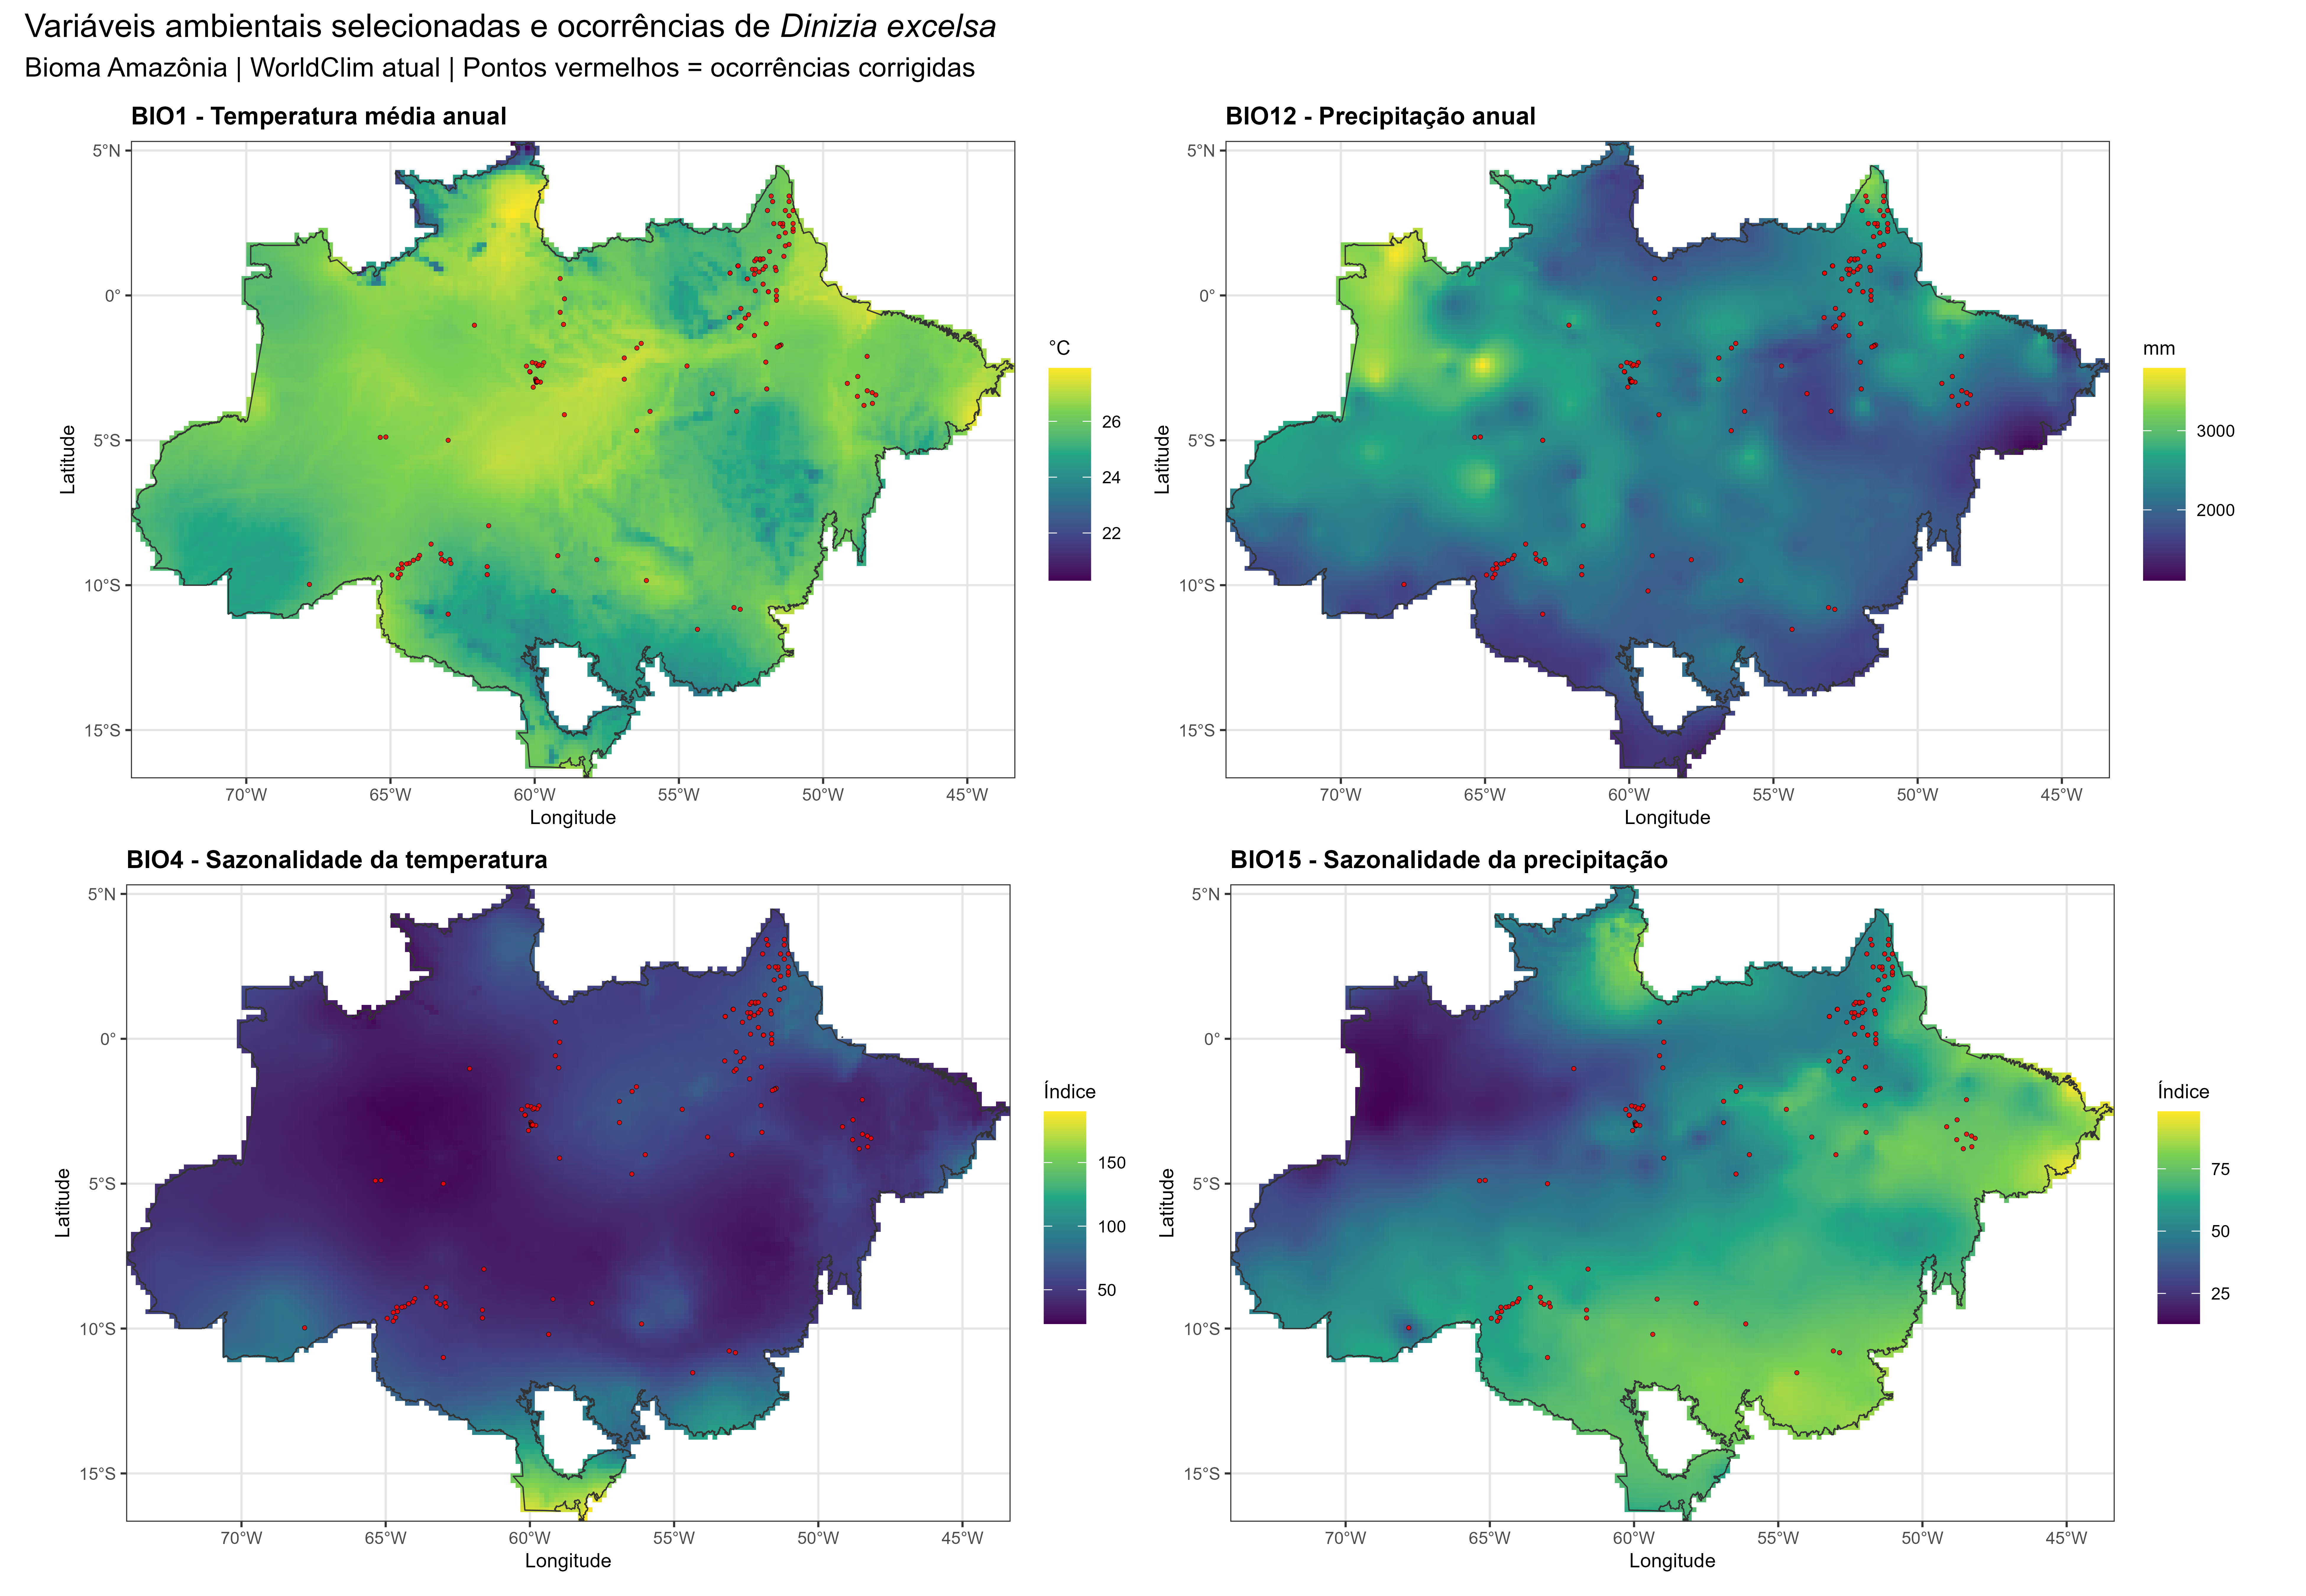
\includegraphics[width=0.96\textwidth]{figuras/unidade01/unidade01_mapas_variaveis_patchwork_dinizia.png}
  \caption{Selected environmental variables across the Amazon biome and corrected records of \textit{Dinizia excelsa}. Each panel uses an independent color scale to show mean annual temperature, temperature seasonality, annual precipitation, and precipitation seasonality.}
  \label{fig:unidade01_variaveis_patchwork_dinizia}
\end{figure}

\begin{figure}[H]
  \centering
  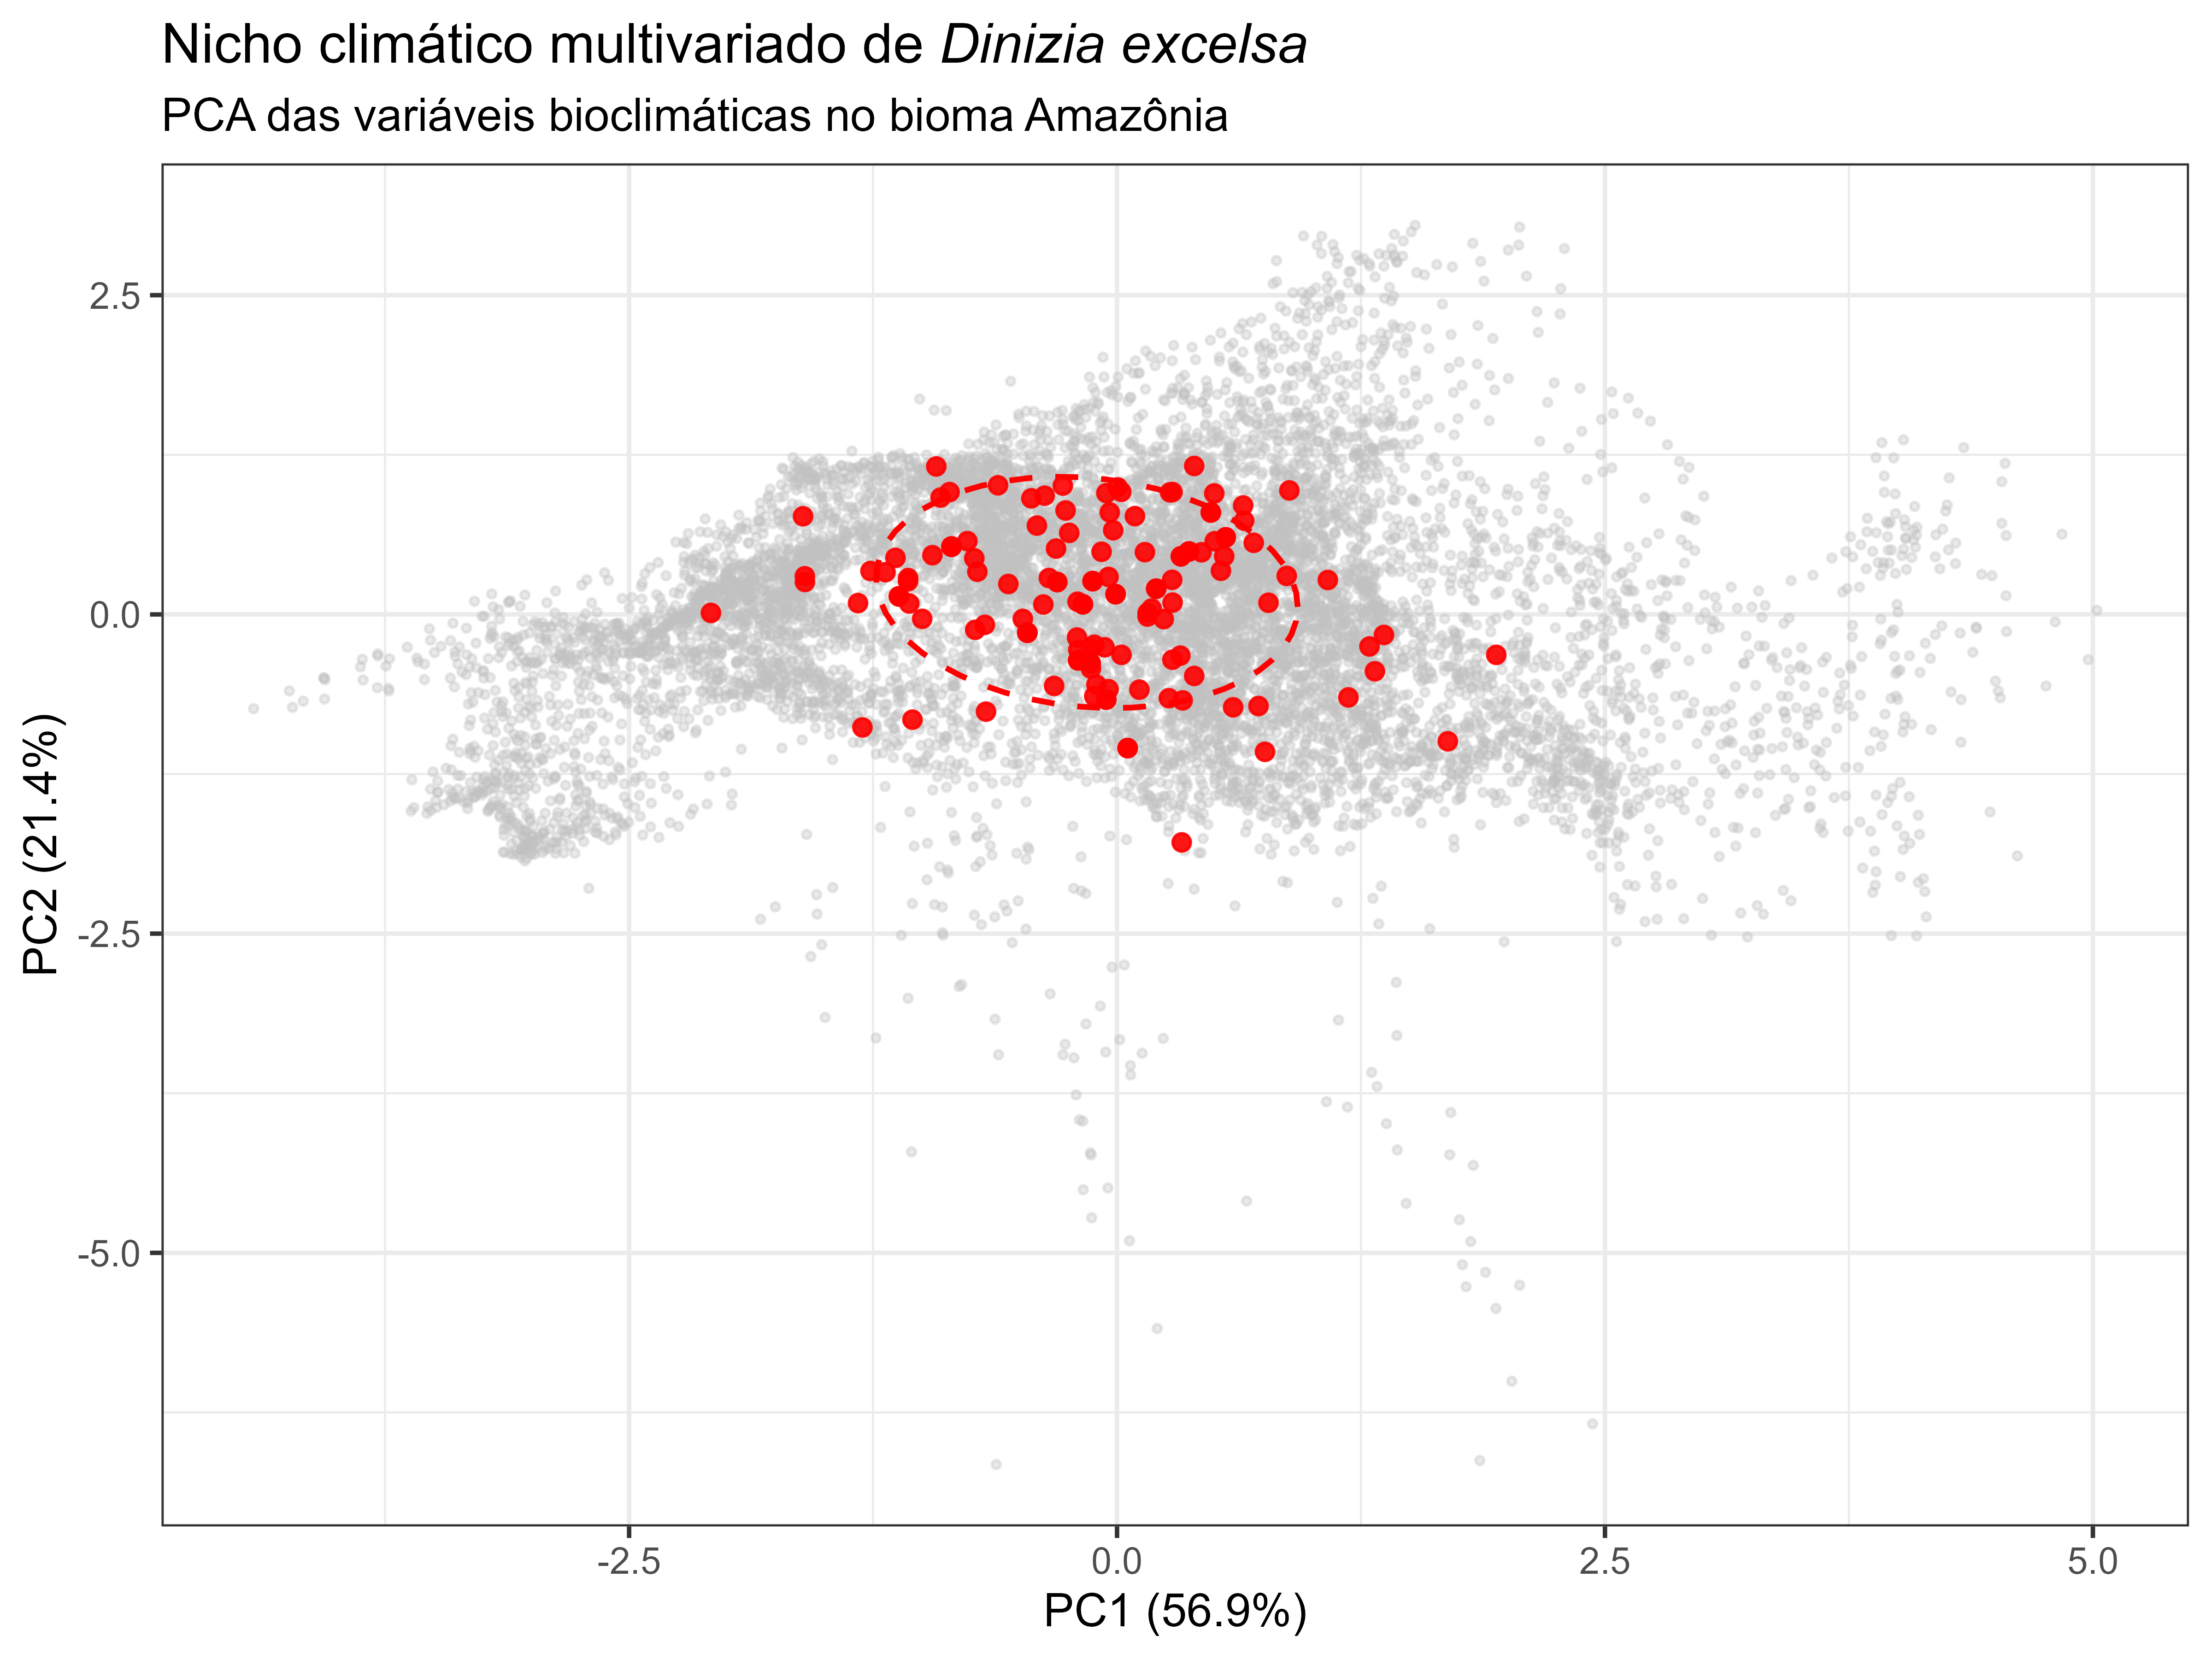
\includegraphics[width=0.82\textwidth]{figuras/unidade01/unidade01_pca_nicho_climatico_dinizia.png}
  \caption{Multivariate climatic niche of \textit{Dinizia excelsa}, represented by a PCA of the selected bioclimatic variables. Gray points represent the environmental background of the Amazon biome; red points are species occurrences.}
  \label{fig:unidade01_pca_dinizia}
\end{figure}

\begin{figure}[H]
  \centering
  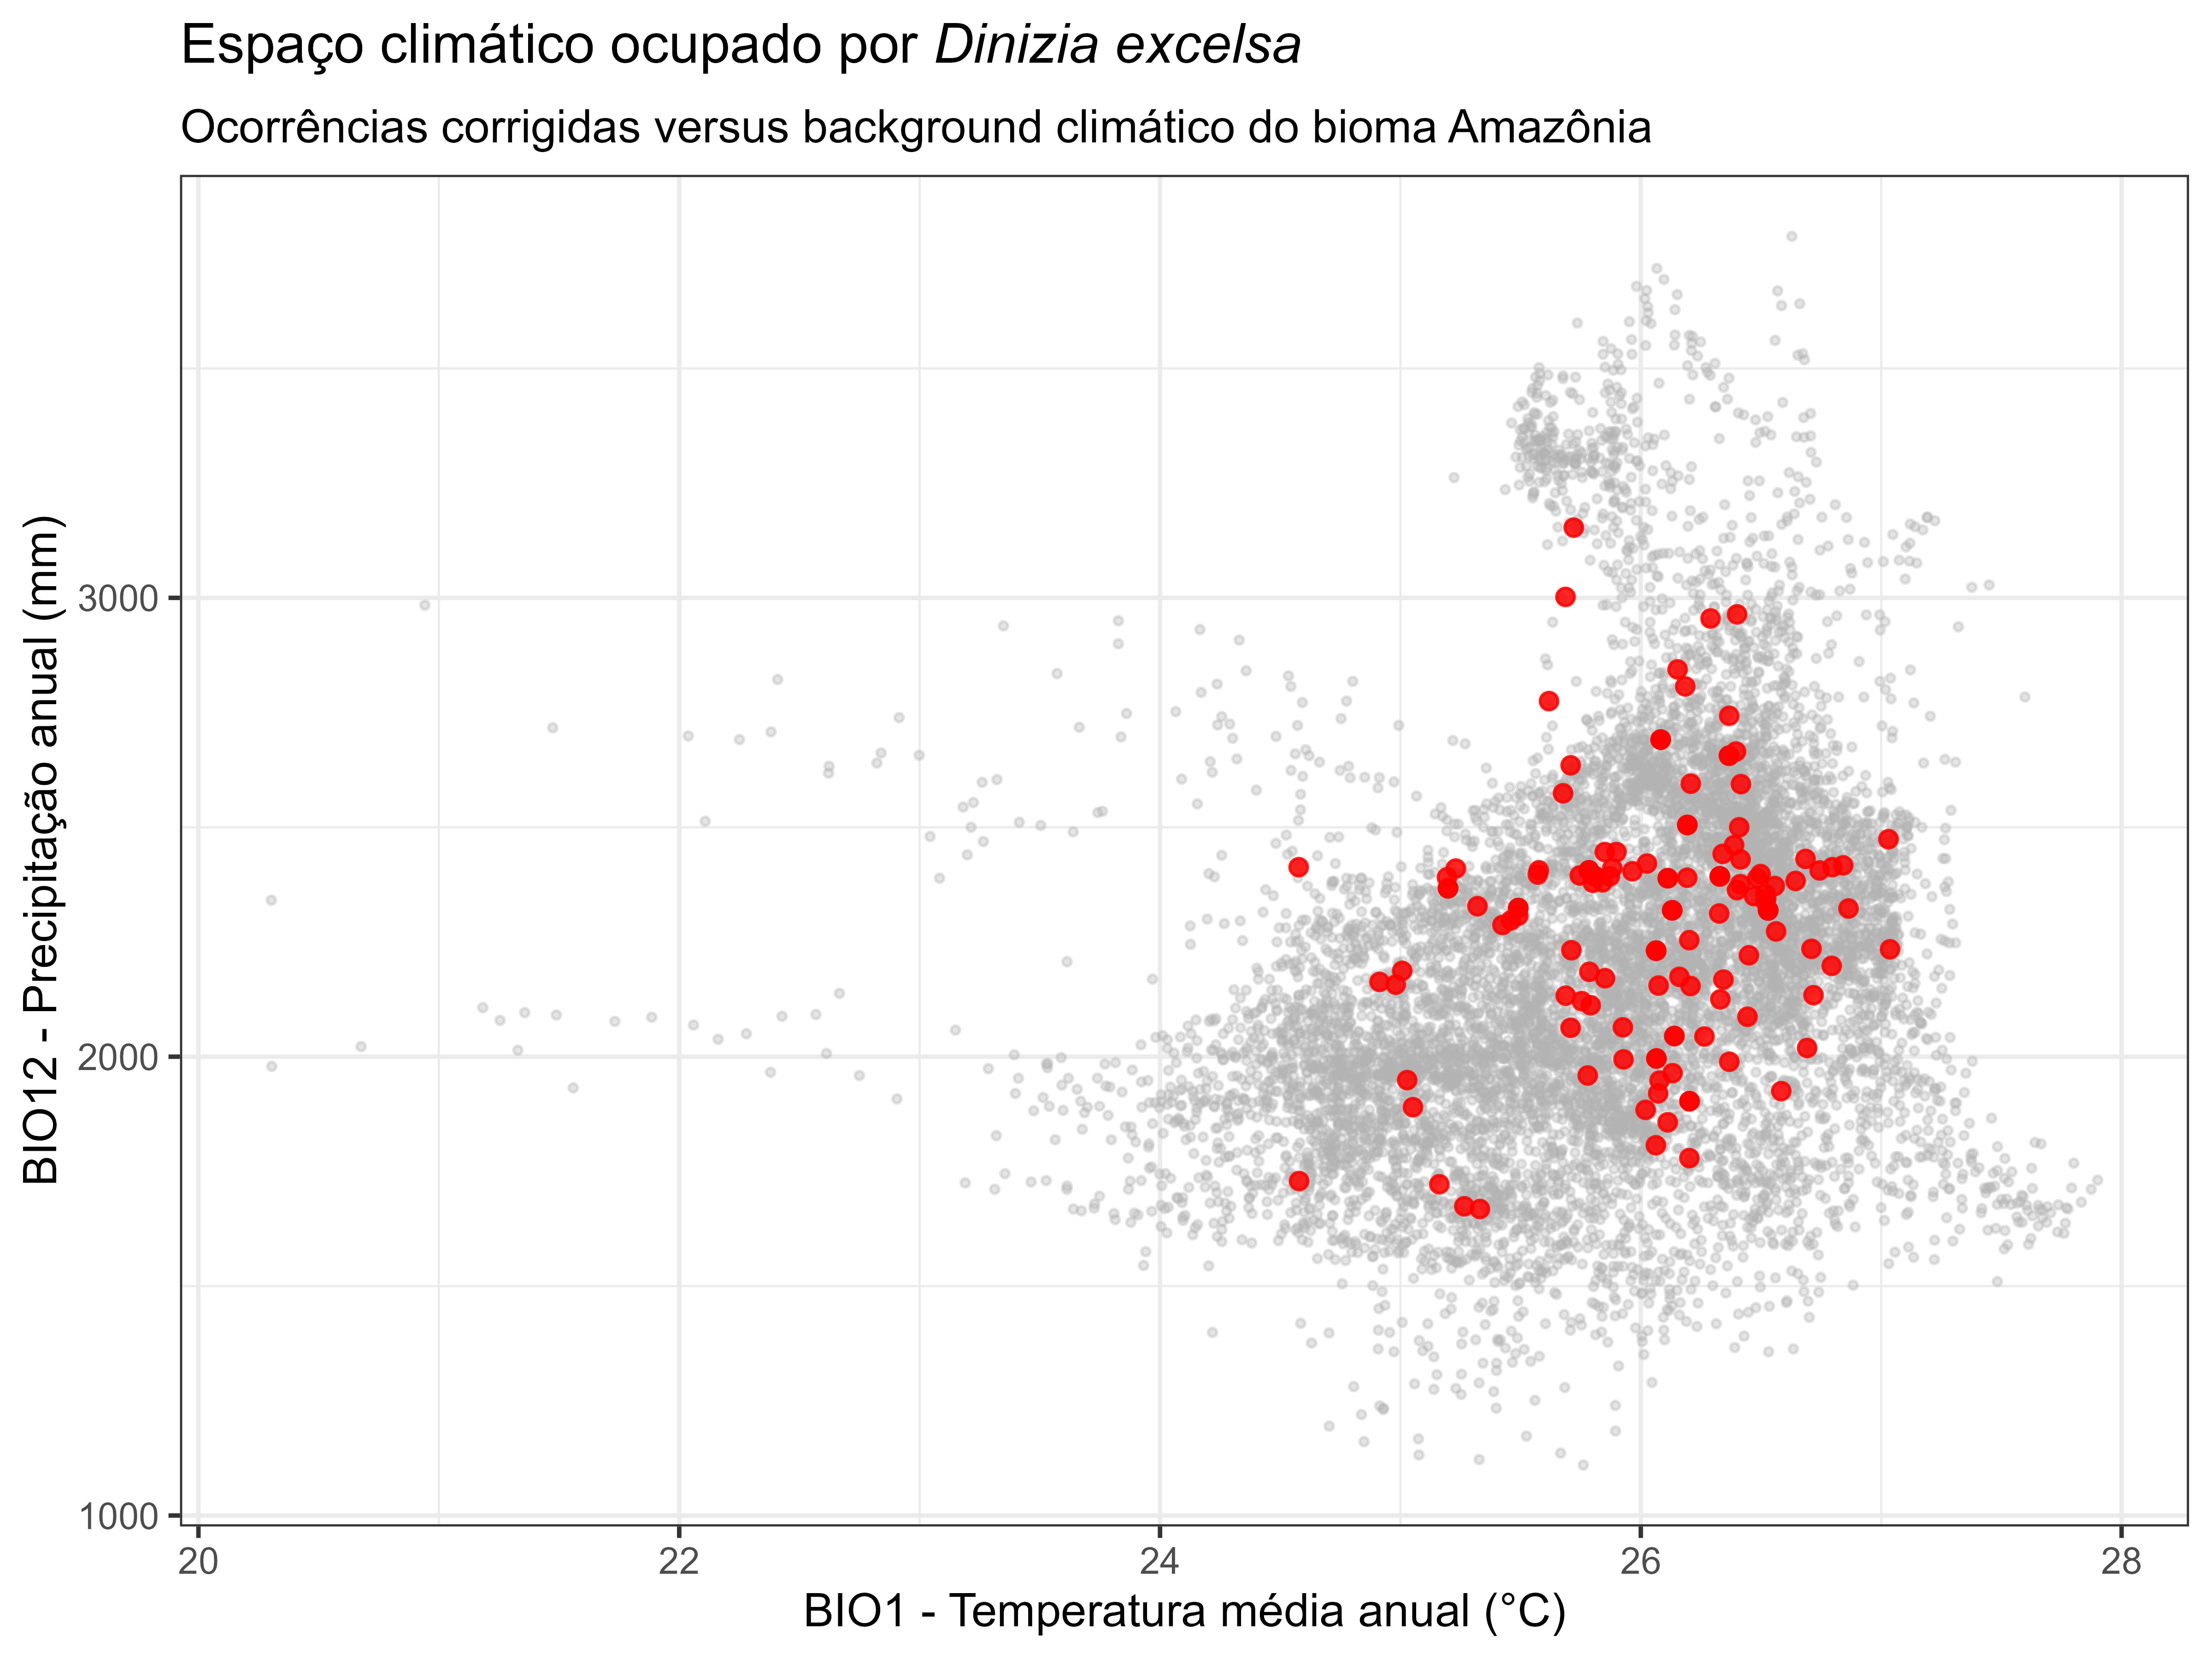
\includegraphics[width=0.82\textwidth]{figuras/unidade01/unidade01_nicho_temperatura_precipitacao_dinizia.png}
  \caption{Climatic space occupied by \textit{Dinizia excelsa} relative to the environmental background of the Amazon biome, based on mean annual temperature and annual precipitation.}
  \label{fig:unidade01_nicho_tp_dinizia}
\end{figure}

\begin{aplicacao}
Figures~\ref{fig:unidade01_pca_dinizia} and
\ref{fig:unidade01_nicho_tp_dinizia} show that the geographic distribution of
\textit{Dinizia excelsa} is associated with a specific subset of the climatic
conditions available across Amazonia. The bivariate plot shows occupation of
the climatic space defined by mean annual temperature and annual precipitation,
whereas the PCA represents the species in a multidimensional environmental
space. Occurrences are concentrated within a more restricted environmental
region than the full background, suggesting ecological filtering related to
the species' climatic requirements. In SDM, these relationships underpin niche
estimation and the projection of potentially suitable areas under present,
past, or future conditions.
\end{aplicacao}

\begin{exercicios}
\begin{enumerate}
  \item Explain the differences among the Grinnellian, Eltonian, and Hutchinsonian niches.
  \item Why do occurrence-based distribution models generally approximate the realized niche rather than the fundamental niche?
  \item Distinguish observed, actual, and potential distributions.
  \item Why should the absence of a biodiversity record not automatically be interpreted as ecological absence?
  \item Discuss the importance of niche conservatism for future climate projections.
  \item For large Amazonian tree species, which factors might cause the distribution of adults to misrepresent the potential distribution of recruits?
\end{enumerate}
\end{exercicios}
